\chapter{Elméleti háttér}

Ahhoz, hogy kellőképpen megértsük a dolgozat által felvetett problémákat, úgy gondolom, hogy szükséges azokat megfelelően, matematikailag tisztán megalapozni. Célom precízen kimondani a megoldandó problémákat, valamint a rájuk alkalmazott különféle technikákat.

\section{Utazóügynök probléma \cite{alg_optim}}
Az utazóügynök probléma (Travelling Salesman Problem, továbbiakban: TSP)  egy fajta optimalizációs probléma, mely során egy járműnek minél rövidebb úton kell megtennie körutat egy adott ponthalmazon. 

Precízen fogalmazva: Adott a bemeneten egy G=(V,E) (irányított) gráf, \[n = |V(G)|, n > 2 \] az állomások száma (a kiindulási állomást beleértve),  \[m = |E(G)| \] az állomások között futó elérhető utak száma.

\[ V = (v_0,v_1, \dots v_n )\]  állomások halmaza (Vertex), \(0 \in V\) a kiindulási állomás,
\[ E = (e_1,e_1, \dots e_m)\] elérhető utak halmaza (Edge),
\[ D : E(G) \mapsto \mathbb{Z}^+\] költségfüggvény (Distance).

A kimenet a legkisebb költségű Hamilton-kör G-re, vagyis azon 
\[ R = (0, v_{i0}, v_{i1} ... 0) \]
bejárás, hogy \( \forall v_i \in V, v_i \in R \) mindegyik csúcsot tartalmazza, és költsége minimális.

A téma a nevét onnan kapta, hogy a XX. században utazó porszívóügynökök autóval járták az Egyesült Államok útjait kereskedés céljából. Az olajválság során megdrágult a járművek működtetéséhez szükséges üzemanyag, és hirtelen megnőtt az igény arra, hogy minél jobban minimalizálják a megtett út hosszát egy-egy üzleti út során. A problémának azóta több alkalmazása is lett, ebből a villamosmérnöki gyakorlathoz egyik legközelebb az SMD beültetőgép bejárása áll. A gép feladata, hogy egy adott nyomtatott áramköri terv alapján lepakolja az alkatrészeket a hordozó lapkára. Az iparban fontos a sebesség, ugyanis ha felére csökkentjük a beültetési időt, akkor akár duplaannyi terméket gyárthatunk le azonos idő alatt. Egy szerelőlemezre alkatrészek százai kerülhetnek, ami nagyon sokféleképpen rendezhető sorba. Természetes igényünk  rövid idő alatt gyors útvonalat találni a beültetőfej számára. A TSP-re \textcolor{red}{KÉPET}. ábrán látható egy látványosabb, vizuális szemléltető példa.

\section{Jármű útvonaltervezési problémák \cite{alg_optim}}
A jármű útvonaltervezési probléma (Vehicle Routing Problem, továbbiakban: VRP) tekinthető a TSP általánosításának. A problémát különböző megkötésekkel lehet feltenni az alkalmazás igénye alapján. Ezek lehetnek például:
\begin{itemize}
	\item járművek maximális száma
	\item az egyes járművek szállítási kapacitása
	\item az egyes helyszínekre történő érkezési idő
\end{itemize}

Feltételezem, hogy ha több jármű van, akkor azok egy közös kezdőpontból (0. pont, raktár, warehouse) indulnak. Útjuk során minden pontot legalább egyszer érinteniük kell a járműveknek, egyazon csúcsba nem szállíthat csomagot két autó. A \ref{VRPpelda}. ábrán látható egy vizuális szemléltető példa.

\begin{figure}[ht!]
	\centering
	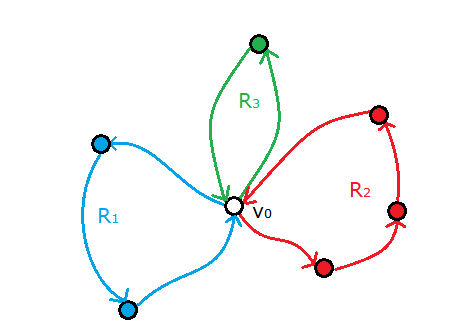
\includegraphics[width=0.5\textwidth]{figures/VRP_Szoveg_nelkul.png}
	\caption{Egy példa VRP végrehajtására n=7 csúcsú gráfon, k=3 járművel \label{VRPpelda} }
\end{figure}

\textbf{Matematikai megfogalmazás :} a problémát gráfokkal modellezhetjük.
\newline 
Legyen G = (V,E) (irányított) gráf, n az állomások száma (a kiindulási állomást beleértve), m az állomások között futó elérhető utak száma, k az elérhető járművek maximális száma.

\[ V = (v_0,v_1, \dots v_n )\]  állomások halmaza (Vertex), \(0 \in V\) a kiindulási állomás,
\[ E = (e_1,e_1, \dots e_m)\] elérhető utak halmaza (Edge),
\[ D : E(G) \mapsto \mathbb{Z}^+\] költségfüggvény (Distance),
\[ L = (l_1,l_2, \dots l_k)\] a járművek szállítási kapacitása (Load capacity),
\[ C : V(G)\setminus \{v_0\} \mapsto \mathbb{R}^+ \] az egyes állomások áruigénye (Claim),
\[ T_{min} :  V(G)\setminus \{v_0\} \mapsto \mathbb{R}^+ \] az egyes állomások készenléti ideje,
\[ T_{max} :  V(G)\setminus \{v_0\} \mapsto \mathbb{R}^+ \] az egyes állomások határideje. Értelemszerűen \(T_{max}(v_i) > T_{min}(v_i) \). A járművek sebessége 1 (tetszőleges egység), az idő és távolság egysége ugyanaz.

Az élek azonosítása érdekében éljünk a következő jelöléssel: e\textsubscript{ij} a v\textsubscript{i}-ből v\textsubscript{j}-be mutató él, és d\textsubscript{i,j} az e\textsubscript{i,j} költsége (itt : távolság, distance). Adott továbbá minden csúcshoz a c\textsubscript{i} áruigény, ami ki kell elégíteni (ez a valóságban lehet db, kg, stb.).Adott minden csúcshoz a c\textsubscript{i} áruigény, amit ki kell elégíteni (ez a valóságban lehet darab, kg, stb. ).  Legyen l\textsubscript{i} az i-edik jármű szállítási kapacitása.

Állítsuk elő útvonalak (Route) olyan \( R_{i} = (0, v_{i_1}, v_{i_2}, \dots 0) \) listáit,
ahol az i-edik jármű azon útvonalát adja meg, amelyet alkotó élek 
\( (e_{0,i_{1}}, e_{i_{1},i_{2}}, \dots e_{i_{m},0}) \). Az útvonal költsége az azt alkotó élek összköltsége. 
\begin{equation}
	c(R_i) = \sum_{v \in R_i} c(v)
\end{equation}


A cél azon \(R_1,R_2,...R_k \) útvonalak megtalálása, amelyekre a következők igazak:
\begin{itemize}
	\item összköltségük minimális
	\item kiindulási és végpontjuk a 0. állomás
	\item a kiindulási csúcsot leszámítva minden csúcsot pontosan egyszer tartalmaznak, vagyis \(\forall v_i \in V, v_i\ne v_0\) esetén \( \exists!R_j : v_i \in R_j \). 
	\item egyik jármű sem szállíthat több árut a megengedettnél, vagyis \(l_i \geqslant \sum_{v \in R_i} c(v) \)
	\item a járművek mindegyik állomásra időben megérkeznek: \(\forall v_i \in V, v_i\ne v_0\) esetén \( T_{min}(v_i) \leqslant t(v_i) \leqslant T_{max}(v_i) \)
\end{itemize}


\paragraph{Hangyakolónia algoritmus \cite{alg_optim}}
Az előbben ismertetett problémákra az optimális megoldás megtalálása NP-nehéz feladat, emiatt nagy csúcs- és élhalmaz mellett nem gazdaságos a kiszámítása. Annak érdekében, hogy a 
gyakorlatban használható algoritmust konstruáljunk, valamilyen közelítő, heurisztikus megoldást érdemes használni a direkt algoritmusok helyett. A hangyakolónia algoritmus (Ant Colony Optimization, továbbiakban: ACO) egy heurisztikus alapelv, mely amellett, hogy képes az optimálishoz nagyon közeli megoldásokat biztosítani, alkalmas a nagyfokú párhuzamosításra. Utóbbi tulajdonsága miatt alkalmas az NVIDIA\textsuperscript{TM} CUDA architektúrájával történő, GPU alapú adaptálásra.

Az eljárás a nevéből adódóan a hangyák (Formicidae) természetben is megfigyelhető élelemkeresési módszerén alapszik. Az első hangyák véletlenszerű (random) útvonalakon haladva keresik az élelemhez vezető utat, majd a visszaúton feromonnal jelölik meg az útjukat. Ezt szagolva a többi hangya későbbmár megfontoltabb döntést hozhat a bejárást illetően. A hátrahagyott feromon erőssége idővel gyengül (modellezhető exponenciális lecsengéssel), ezzel biztosítva, hogy a nem optimális útvonalak (az élelemhez vezet, de már van nála rövidebb) maguktól elhaljanak. Látható, hogy olyan él, ami sok ideig nem kap feromon utánpótlást, exponenciális jelleggel lecseng.

Az algoritmus futása során nyilvántartunk egy feromongráfot. A feromongráf és az eredeti gráf topológiája megegyezik, de az élek súlyozása eltérő. Legyen Ph(V,E) gráf, amiben az élek súlyai \( e_{i,j} \rightarrow \tau_{i,j} \) .

Gráfbejárás során egy \(v_i\)-n álló hangya a továbblépéséhez a lehetséges kimenő élek közül a feromon és és az élsúly alapján "céltábla elv szerint", véletlenszerűen választ. Az egyes élek kiválasztásának valószínűsége
\begin{equation}
	P_{i,j} = \frac{(\tau_{i,j})^\alpha(d_{i,j})^\beta}{\sum_{l \in N_i^k}(\tau_{i,l})^\alpha(d_{i,l})^\beta }
	\label{ACO_General_probability}
\end{equation}


ahol \(N_i^k \) az algoritmus k-adik lépésében az i-edik csúcsból elérhető szomszédos csúcsok halmaza. Az \(\alpha\) és \(\beta\) a feromonok és élsúlyok figyelembevételét szabályozza. Például minél nagyobb valahol a feromon, annál inkább akarunk oda továbbmenni, illetve minél messzebb van egy adott pont, annál inkább el akarjuk kerülni. Saját megvalósításom esetén gyorsítás céljából elhanyagoltam ezen ponton az élhosszak figyelembe vételét, ezért \(\beta = 0\). Továbbá az egyszerűség kedvéért legyen \(\alpha = 1\). Ennek az az előnye, hogy a \ref{ACO_General_probability}. egyenlet a következővé egyszerűsödik:
\begin{equation}
	P_{i,j} = \frac{\tau_{i,j}}{\sum_{l \in N_i^k}\tau_{i,l}}
	\label{ACO_My_probability}
\end{equation}

Miután minden hangya végigment egy úton (legenerált egy csúcssorrendet, legyen az akár lehetséges, akár nem) értékeljük az útvonalakat. A teljesíthető útvonalak esetén a élek feromonszintjét a útvonal hosszával fordítottan arányosan \(\beta = -1\) megnövelem. Ez biztosítja, hogy a rövidebb útvonalak nagyobb feromonszinttel rendelkezzenek, ezáltal több hangya menjen előbb-utóbb olyan irányba. 

Az éleken található feromon növelése után mindegyik élt exponenciális jelleggel csökkentem: minden feromon gyengül egy előre beállítandó, konstans szorzóval, ez a párolgás \(\rho\). Összességével minden iteráció végén a következő történik egy él feromonjával:
\[ \tau_{i,j} \leftarrow (1-\rho)\tau_{i,j} + \Delta\tau_{i,j} \]

Az útkeresés közben mindig fel kell jegyezni a legjobb addigi megtalált utat. Az ACO algoritmus egyik előnye, hogy több, hasonlóan jó alternatív utat is képes megtalálni. Ez például térképes útvonaltervezésnél lehet hasznos. Az algoritmus javítása érdekében bevezettem, hogy az a hangya, aki minden korábbinál rövidebb utat talál, az egy ún. "Jutalom szorzó"-t kap. Ez azt jelenti, hogy a feromonjához adandó többlet a szorzószorosára változik, így a következő iterációban sokkal nagyobb valószínűséggel fog arra menni a jövő hangyája. Ez a jutalmazási rendszer rossz beállítások mellett kezdetben félreviheti a hangyákat egy rossz útvonal felé, ezért állítható, hogy hányadik iterációtól kezdve kaphassanak az útvonalak "Jutalom szorzó"-t.

\section{Alternatív megoldások}

Dolgozatomban főleg a Hangyakolónia algoritmussal foglalkoztam, de nem azt jelenti, hogy ez az egyetlen járható út. Nézzünk meg néhány alternatív kiindulási gondolatot.

\subsection{„Brute force” algoritmus}
A „Brute force” algoritmus lényege, hogy minden lehetséges bejárást megvizsgálunk, és kiválasztjuk a legrövidebb, a konkrét probléma feltétel(rendszer)ének eleget tevő esetet. \textbf{Ha n db csúcs}ból álló teljes gráfot nézünk (mint ahogy ez a valóságban igen gyakori), \textbf{akkor n! különböző lehetséges bejárás}t kell összehasonlítani. Kis n esetén még csak-csak elfogadható ez a módszer, viszont ha már csak pl. \(n=48\) db csúcsunk van (mert esetleg szeretnénk bejárni TSP szerint az Amerikai Egyesült Államok 48 összefüggő államának fővárosait, később lesz rá példa), a vizsgálandó esetek száma felugrik \( 48! \approx 1.24 * 10^{61} \)-re. Tegyük fel, hogy csúcskategóriás, 5GHz-en pörgő szuperszámítógépünk képes átlagosan 1 órajelciklusonként (  \(2*10^{-10}s\) időközönként, nagyjából lehetetlenül gyorsan) kiszámolni egy út hosszát, még így is kb. \(2.5 * 10^{51}s \approx 8 * 10^{43} \) évig vizsgálhatnánk az eseteket. Egy SMD beültetőgép egy szerelőlemezre akár alkatrészek százait pakolhatja fel, ilyen módszerrel lehetetlen lenne megmondani, hogy milyen sorrendben haladjon. Látható tehát, hogy ha véges időn belül meg akarjuk oldani a problémát, ravaszabbnak kell lennünk.

\subsection{Held-Karp algoritmus }
A Held-Karp algoritmust M. Held és R. Karp urak alkották meg 1962-ben \cite{HeldKarp}. Azért beszédes ez az évszám, mert ekkoriban kezdett magának teret hódítani a számítástudomány, és ekkor készültek el az első számítógépek. Módszerük, hogy egyesével, rendezetten szúrnak be csúcsokat egy egyre növekvő ponthalmazba. Hasonlít a beillesztéses rendezésre, csak kicsit komplexebb. Kihasználja, a korai számítógépek képesek voltak már rekurzív programok futtatására.
\paragraph{}
Jelöljük a csúcsokat \( V=\left(v_1,v_2,\ldots v_n\right) \) -nel, \(v_1\) önkényesen kijelölhető kezdőpontnak. Legyen S halmaz a csúcsok valamely részhalmaza: \(S \subseteq \{v_2,...v_n\}\). Legyen g(S,e) \(v_1\)-ből az S összes elemén keresztül az e \(\neq v_1\)  csúcsba végződő legrövidebb út hossza. Az u-ból a v-be mutató él költsége d(u,v).
Lépésenként kiszámítjuk a g(S,e) értékeket kezdte a kis S-ekkel.

Példák:
\begin{itemize}
	\item \(\forall e: g(\emptyset,e) = d(1,e)\)
	\item \(g(\{2\},4)\) csak az összhossza az  \(1 \rightarrowtail 2 \rightarrowtail 4\) útnak
	\item \(g(\{2,3\},4)\)  az ( \(1 \rightarrowtail 2 \rightarrowtail 3 \rightarrowtail 4\) ) és ( \(1 \rightarrowtail 3 \rightarrowtail 2 \rightarrowtail 4\) ) utak rövidebbikének a költsége
\end{itemize}

Amikor már 3 vagy több pontot tartalmaz az S halmaz, a lehetséges utak száma drasztikusan megnő, de csak néhányat kell figyelembe venni a legrövidebb út keresése érdekében. Vegyük észre, hogyha az (\(1\rightarrowtail 4\rightarrowtail 3\rightarrowtail 2\)) út rövidebb, mint az (\(1\rightarrowtail 3\rightarrowtail 4\rightarrowtail 2\)), akkor az (\(1\rightarrowtail 4\rightarrowtail 3\rightarrowtail 2\rightarrowtail 5\)) út is rövidebb lesz, mint a (\(1\rightarrowtail 3\rightarrowtail 4\rightarrowtail 2\rightarrowtail 5\)).
\paragraph{}
Általánosan: tegyük fel, hogy a k-adik lépésben \(S=\{s_1,...s_k\}\). Jelöljük \(1\leqslant i\leqslant k\)-ra \(S_i = S-\{s_i\} = \{s_1...s_{i-1},s_{i+1}...s_k\} \). Ha a \(v_1\)-ből a legrövidebb út e-be S-en keresztül úgy vezet, hogy annak \(s_i\) az utolsó előtti eleme, akkor következik, hogy \(v_1\)-ből a legrövidebb út \(s_i\)-be \(S_i\)-n keresztül vezet. Ez azt jelenti, hogy a k-adik lépésben elég k db S halmazt továbbvinnünk, mert csak azok lehetségesek legrövidebb utat adni.

\subsubsection{Az eljárás Értékelése}
A Held-Karp algoritmus exponenciális idejű, \(O(2^nn^2)\), ami nagyságrendekkel jobb, mint a brute-force módszer az ő \(O(n!)\) faktoriális idejével. Előnye a Hangyakolónia algoritmussal szemben, hogy determinisztikus algoritmus révén a végén mindig a legrövidebb utat adja eredményül. Hátránya azonban, hogy rekurziót alkalmaz, ami gyakran kedvezőtlen programvégrehajtás szempontjából (sok rekurzív függvényhívás megterheli a stacket). Egyéb észrevétel, hogy ha különböző feltételekkel keresünk utakat, akkor az algoritmus elveszíti alapelvét, nem elég mindig az előző ciklus legjobbjaiból kiindulni. Ezzel a problémával az ACO is szembesül, de kevésbé van rá kihatással.